\begin{figure}[h!]
	\centering{
		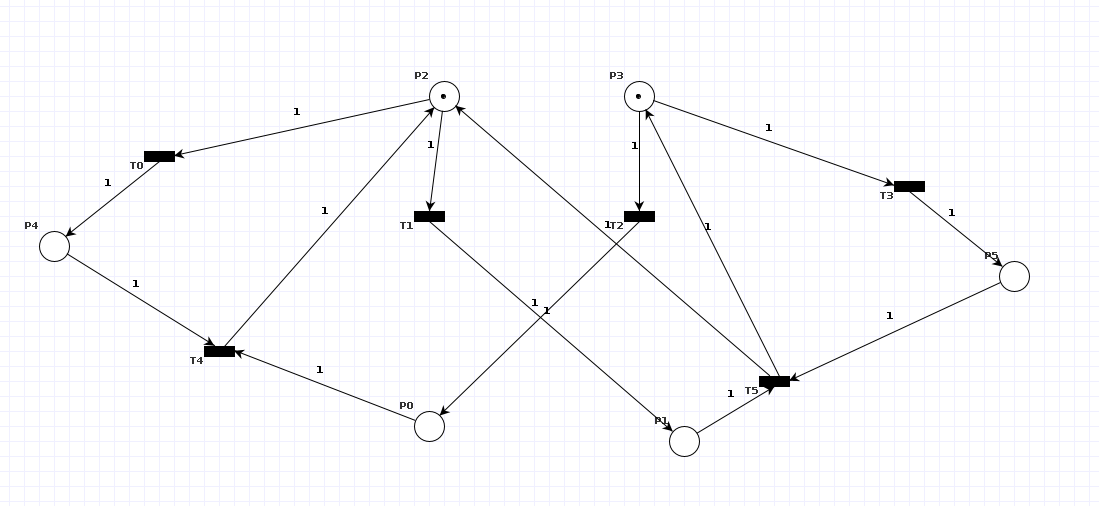
\includegraphics[width=0.67\textwidth]{img/d.png}
	}
	\caption{Sieć z deadlockiem}
	\label{zad2:graph1}
\end{figure}

\begin{figure}[h!]
	\centering{
		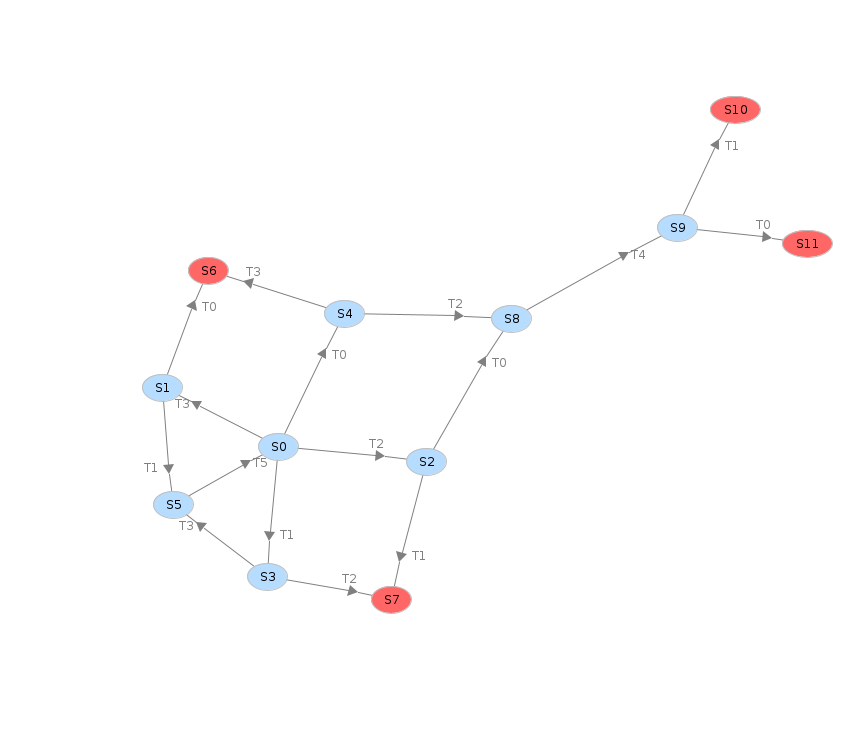
\includegraphics[width=0.67\textwidth]{img/dr.png}
	}
	\caption{Graf osiągalności}
	\label{zad2:graph1}
\end{figure}
\begin{figure}[h!]
	\centering{
		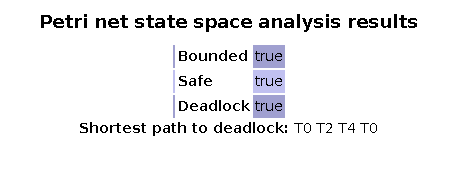
\includegraphics[width=0.67\textwidth]{img/dd.png}
	}
	\caption{Niezminniki sieci}
	\label{zad2:graph1}
\end{figure}

\subsection{Graf osiągalności}
Jak widzimy graf osiągalności posiada sekcje z których nie da się wyjść 
(zaznaczone na czerowno). Gdy sieć wchodzi do tego stanu następuje zakleszczenie.

\subsection{Analiza przestrzeni stanów}
Obecność zakleszczenia możemy także zaobserwować w tabeli analizującej 
przestrzeń stanów naszej sieci.